\documentclass[a4paper, 10pt]{article}
    \usepackage[subpreambles=true]{standalone}
    \usepackage[english, american, british]{babel}
    \usepackage[utf8]{inputenc}
    \usepackage[T1]{fontenc}
    \usepackage{hyphenat}
    \hyphenation{Mathe-matik wieder-gewinnen}
    \usepackage{amsmath}
    \usepackage{import}
    \usepackage{tabularx}
    \usepackage{graphicx}
    \usepackage[margin=2cm ]{geometry}

    \title{Einführung in die Softwaretechnik 2018 \\ Sheet 05}
    \author{Maximilian Frühauf}

\begin{document}
\maketitle
\begin{enumerate}
    \item
    Explain the difference between a 3-layered architectural style and a 3-tier architecture.
    \vspace{0.5cm}

    A 3-layered architecture is a system that has 3 hierarchically ordered layers in the model.
    Each of these builds on top of the next and can be realized with an open or closed architecture.
    An example for this would be a basic GUI application where all user interaction is handled on the 
    View layer. This input is then passed on to various Controller(s) to be processed. If any of the 
    internal state of the application needs to be changed as a result, the Model layer is updated.


    A 3-tier architecture however is also divided into three separate layers, but these are then 
    distributed to three different physical systems.
    This architecture style is for example present in most modern web applications, where the first 
    tier is the user's web browser. It then connects to the application's web server and 
    receives html, css and JavaScript files. If any state needs to be saved or loaded the 
    third tier is invoked. This is the database backing the web server.
    \item
    Create a UML component diagram for Bumpers based on the following analysis object model. 
    Use the Model View Controller (MVC) architectural style and explain why you modeled it like this.
    \vspace{0.5cm}
    
    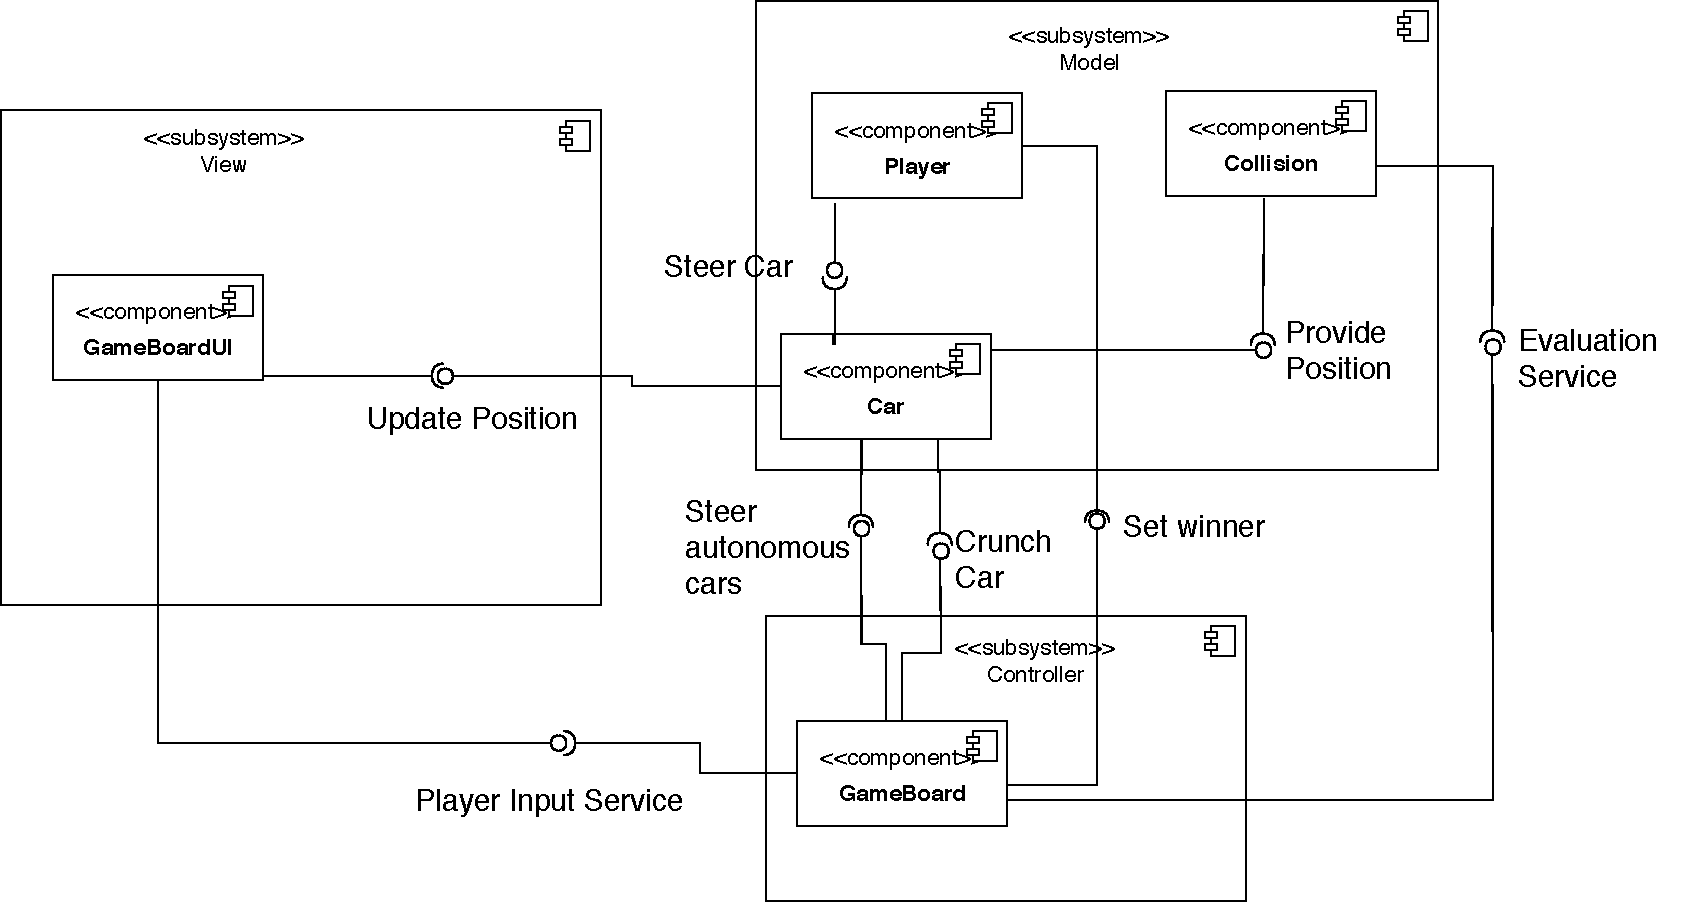
\includegraphics[width=\linewidth]{task2.pdf}


    \item
    Consider the following extension to Bumpers. 
    The game includes a high- score mechanism to determine the best players. 
    High-scores are saved on a separate database server and are accessed by the game through an 
    application server. To improve redundancy, two identical database servers should be used: 
    the first acts as a main server, and the second acts as a redundant back-up in case the 
    first one fails. The Bumpers game accesses data through the application server. 
    Game administrators have the option of using a proprietary client that accesses the databases 
    directly. Draw a UML deployment diagram representing the hardware/ software mapping of this 
    system and explain why you modeled it like this. Which architectural style did you choose?
    \vspace{0.5cm}


    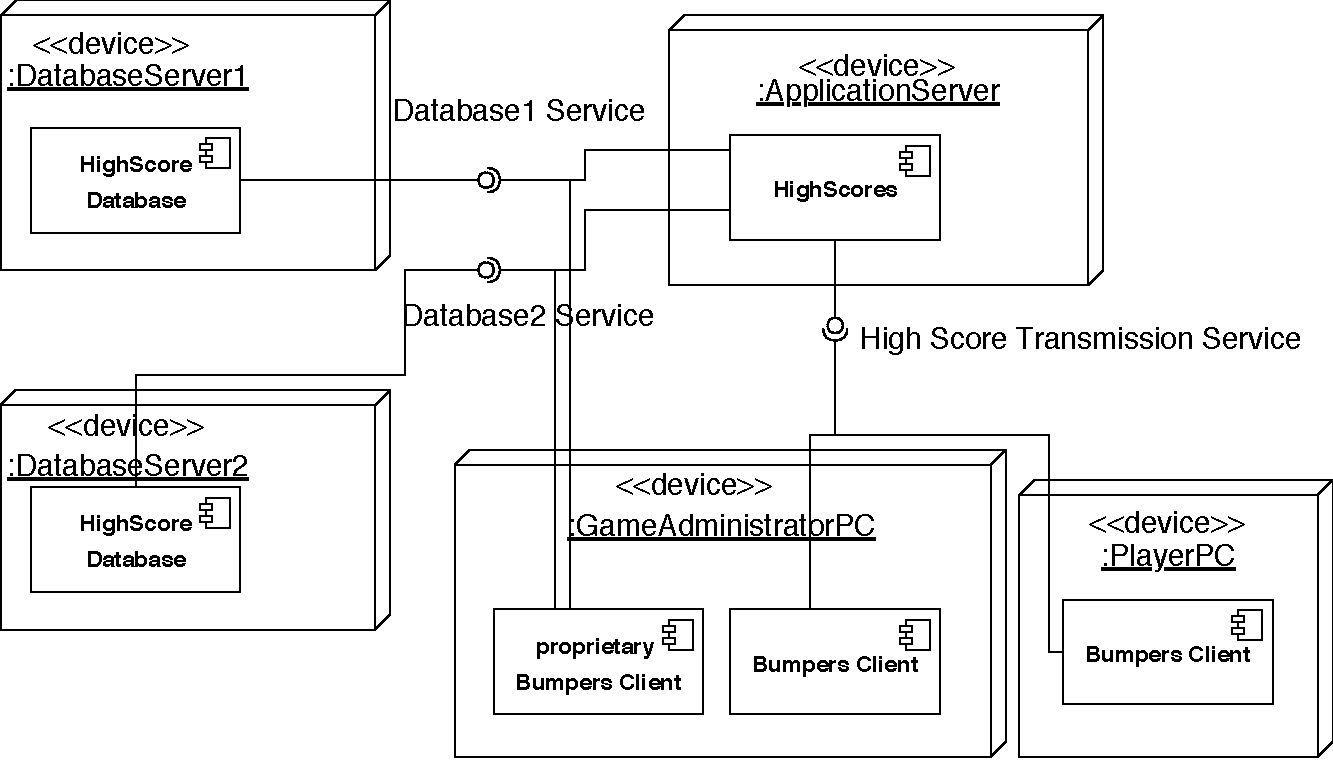
\includegraphics[width=\linewidth]{task3.pdf}


    The architectural style chosen is a 3-tiered architecture.
    \item
    Consider a legacy, fax-based, problem-reporting system for an aircraft manufacturer. 
    You are part of a reengineering project replacing the core of the system with a 
    computer-based system that includes a database and a notification system. 
    The client requires the fax to remain an entry point for problem reports. 
    You propose an E- mail entry point. Describe a subsystem decomposition that would allow 
    both interfaces. Note that such systems are used to process many problem reports per 
    day (e.g., 2000 faxes per day). Draw a UML component diagram representing the 
    subsystem decomposition of this system and explain why you modeled it like this.
    \vspace{0.5cm}

    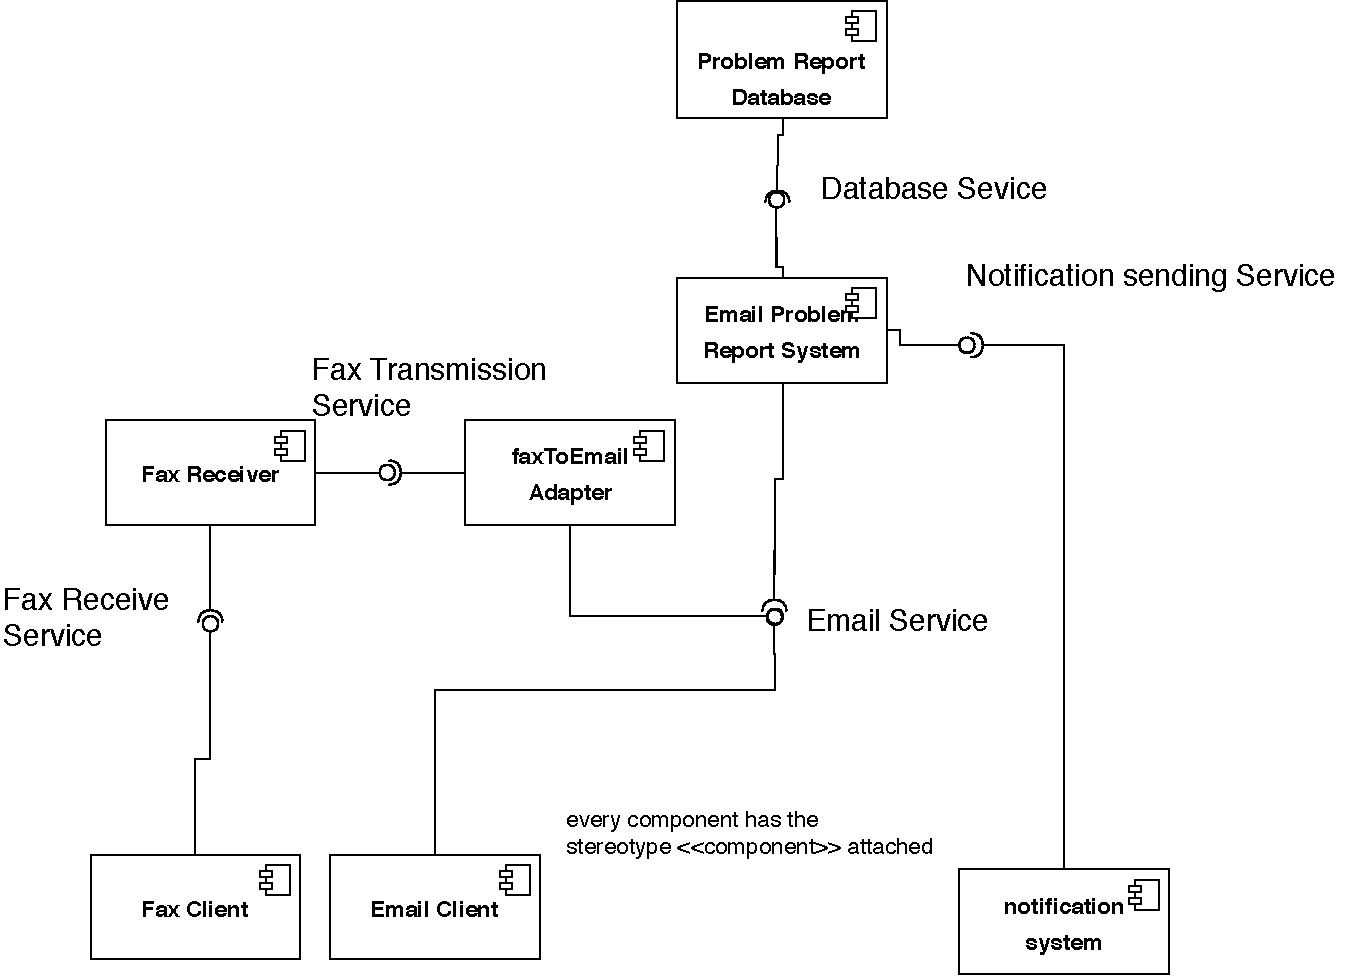
\includegraphics[width=\linewidth]{task4.pdf}
\end{enumerate}
\end{document}